% flashcards-title: The same twelve counters in two different rectangular arrays
% flashcards-desc: Twelve counters shown twice. The first arrangement is a rectangular array with fewer, longer equal rows. The second arrangement is a different rectangular array with more, shorter equal rows. No row or column counts are labeled and no statements are shown.
\documentclass[tikz]{standalone}
\usetikzlibrary{arrows.meta,patterns}

\definecolor{qraNavy}{HTML}{17324D}
\definecolor{qraBlue}{HTML}{2B6CB0}
\definecolor{qraGold}{HTML}{B7791F}
\definecolor{qraPale}{HTML}{EAF2F8}
\definecolor{qraGray}{HTML}{5C6773}

\tikzset{
  qra axis/.style={draw=qraNavy, line width=1.2pt},
  qra tick/.style={draw=qraNavy, line width=1pt},
  qra guide/.style={draw=qraGray, densely dashed, line width=0.8pt},
  qra counter/.style={circle, draw=qraNavy, fill=qraPale, line width=0.9pt, minimum size=7mm, inner sep=0pt},
  qra label/.style={font=\sffamily\bfseries, text=qraNavy},
  qra small label/.style={font=\sffamily, text=qraNavy},
}

\begin{document}
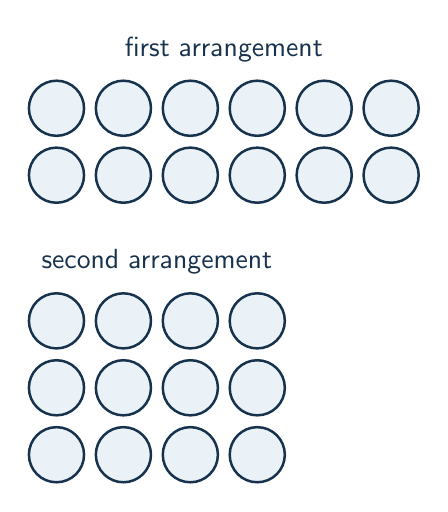
\begin{tikzpicture}
  % First array: 2 rows x 6 columns
  \foreach \i in {0,...,5}
    \foreach \j in {0,1}
      \node[qra counter] at (\i*0.85, -\j*0.85) {};
  \node[qra small label] at (2.125, 0.75) {first arrangement};

  % Second array: 3 rows x 4 columns
  \foreach \i in {0,...,3}
    \foreach \j in {0,1,2}
      \node[qra counter] at (\i*0.85, -\j*0.85 - 2.7) {};
  \node[qra small label] at (1.275, -1.95) {second arrangement};
\end{tikzpicture}
\end{document}
